%
% Chapter 3 - System Architecture and Data Model
%
\chapter{System Architecture and Data Model} \label{cap:architecture}

To ensure the project's viability, maintainability, and security, the architecture was designed around technologies that are widely adopted in the industry and that allow the application to be hosted within ISEL's own infrastructure.

\section{Global System Overview} \label{sec:system-overview}

EduCal follows a three-tier architecture that separates presentation, business logic, and data storage.

\begin{figure}[htbp]
\begin{center}
\resizebox{115mm}{!}{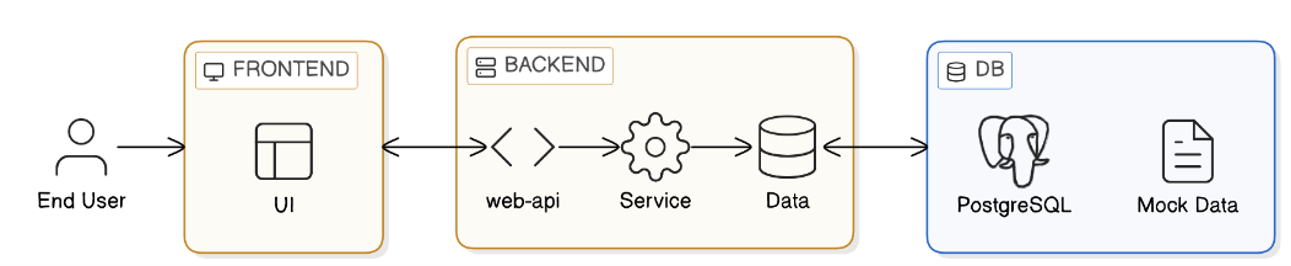
\includegraphics{./figures/system_architecture.png}}
\end{center}
\caption{System architecture diagram.}\label{fig:architecture}
\end{figure}
\FloatBarrier

As illustrated in Figure~\ref{fig:architecture}, the system is organized into three layers:

\begin{itemize}
    \item \textbf{Presentation Layer (Frontend):} built with Next.js and React, manages the complex calendar views (Agenda, Day, Week, Month, Year) and specialized interfaces for event/occurrence management, such as dynamic multi-occurrence forms.
    \item \textbf{Logic Layer (Backend):} Next.js API routes backed by a Controller-Service-Data structure (Chapter~\ref{cap:backend}): controllers parse and validate requests, services hold the core business logic and enforce role-based access (the Migration Engine, RF02, and Business Rule Engine, RF03), and the data layer abstracts all storage communication.
    \item \textbf{Data Layer (DB):} a PostgreSQL relational database provides persistent storage for events, occurrences, and system configuration, accessed through the Drizzle ORM.
\end{itemize}

All components outlined here have been implemented, including PostgreSQL, so far tested only against a local instance (Chapter~\ref{cap:deployment}). The data access layer isolates all storage behind a single point in the code, so business services never talk to the database directly, which is what makes it possible to keep an alternative JSON-based backend, currently used for the Vercel preview deployment, without any changes to the business logic, API routes, or frontend (Section~\ref{sec:data-access}).

\section{Technology Stack} \label{sec:tech-stack}

The stack was chosen to keep the whole application, frontend and backend alike, in a single TypeScript codebase, avoiding the coordination overhead of separate languages or repositories for a project of this size.

\subsection{Backend}
The backend is built on \textbf{Next.js}~\cite{nextjs} (v16, App Router), using its API routes as the HTTP entry point rather than a separate server framework. Data persistence uses \textbf{PostgreSQL}~\cite{postgresql} through \textbf{Drizzle ORM}~\cite{drizzleorm}, a TypeScript-first ORM that provides both a relational query API and raw SQL migrations (\texttt{drizzle-kit}). Request payloads are validated end-to-end with \textbf{Zod}~\cite{zod}, including schemas that are built dynamically from live database values (e.g. valid event categories). Password hashing uses Node.js's built-in \texttt{crypto} module~\cite{nodejscrypto} (scrypt), and session cookies follow the \texttt{Secure}/\texttt{HttpOnly} guidance from the OWASP Session Management Cheat Sheet~\cite{owasp}. National holiday and business-day calculations use the \texttt{date-fns} and \texttt{date-holidays} libraries. The automated test suite (Section~\ref{sec:backend-tests}) is built on \textbf{Vitest}~\cite{vitest}.

\subsection{Frontend}
The frontend is built with \textbf{React 19}~\cite{react} inside the same Next.js application (no separate frontend project), styled with \textbf{Tailwind CSS v4}~\cite{tailwindcss} and the \textbf{shadcn/ui}~\cite{shadcnui} component library (built on Radix UI primitives~\cite{radixui}). Forms use \textbf{react-hook-form}~\cite{reacthookform} together with \textbf{Zod resolvers} for validation, \textbf{sonner} provides toast notifications for asynchronous feedback, \textbf{framer-motion}~\cite{framermotion} drives the calendar's animations, the native HTML5 drag-and-drop API handles occurrence rescheduling, and \textbf{re-resizable} handles occurrence resizing. The project uses \textbf{pnpm}~\cite{pnpm} as its package manager and \textbf{TypeScript}~\cite{typescript} throughout both the frontend and backend.

\section{Data Model and Entity-Relationship Diagram} \label{sec:data-model}

To support automated year-to-year migration, rule validation, and the notification system (Section~\ref{sec:backend-notifications}), a relational database schema was designed and implemented with Drizzle ORM, visually outlined in the simplified Entity-Relationship Diagram in Figure~\ref{fig:er-diagram}, generated directly from the Drizzle schema definitions (\texttt{db/schema/auth.schema.ts}, \texttt{db/schema/calendar.schema.ts}, \texttt{db/schema/notification.schema.ts}, \texttt{db/schema/relations.ts}). This diagram shows every table and its relationships but omits column-level attributes for readability; the full version, with every column and its type, is given in Appendix~\ref{app:er-diagram}.

\begin{figure}[htbp]
\begin{center}
\resizebox{\textwidth}{!}{%
\begin{tikzpicture}[
    entity/.style={draw, rectangle, rounded corners=1pt, align=center, font=\small\bfseries, text width=2.8cm, inner sep=2mm, fill=white},
    relationship/.style={draw, diamond, aspect=3.4, font=\small, inner sep=1mm, align=center, fill=white},
    cascade/.style={thick},
    restrict/.style={thick, dashed},
    card/.style={fill=white, inner sep=1.5pt, font=\small},
]

% --- entities ---
\node[entity] (events) at (0,0) {Event};
\node[entity] (academicyears) at (-6,4.5) {Academic Year};
\node[entity] (users) at (6,4.5) {User};
\node[entity] (vacationperiods) at (-6,7.8) {Vacation Period};
\node[entity] (sessions) at (6,7.8) {Session};
\node[entity] (categories) at (-10,-4.5) {Category};
\node[entity] (classifications) at (-4,-4.5) {Classification};
\node[entity] (statuses) at (4,-4.5) {Status};
\node[entity] (responsibles) at (10,-4.5) {Responsible};
\node[entity] (occurrences) at (-2.0,-10) {Occurrence};
\node[entity] (rules) at (2,-10) {Event Rule};
\node[entity] (notifications) at (-2.0,-14) {Notification};

\node[relationship] (rel-ay-events) at ($(academicyears)!0.5!(events)$) {has};
\node[relationship] (rel-ay-vac) at ($(academicyears)!0.5!(vacationperiods)$) {has};
\node[relationship] (rel-users-events) at ($(users)!0.5!(events)$) {creates};
\node[relationship] (rel-users-sessions) at ($(users)!0.5!(sessions)$) {authenticates};
\node[relationship] (rel-events-cat) at ($(events)!0.7!(categories)$) {categorized\_as};
\node[relationship] (rel-events-class) at ($(events)!0.7!(classifications)$) {classified\_as};
\node[relationship] (rel-events-status) at ($(events)!0.7!(statuses)$) {has\_status};
\node[relationship] (rel-events-resp) at ($(events)!0.7!(responsibles)$) {assigned\_to};
\node[relationship] (rel-events-occ) at ($(events)!0.68!(occurrences)$) {has};
\node[relationship] (rel-events-rules) at ($(events)!0.68!(rules)$) {has};
\node[relationship] (rel-occ-notif) at ($(occurrences)!0.5!(notifications)$) {has};

% --- edges: entity -- diamond -- entity, with cardinalities near each entity end ---
\draw[cascade] (academicyears) -- (rel-ay-events) node[card, pos=0.2] {1};
\draw[cascade] (rel-ay-events) -- (events) node[card, pos=0.8] {N};

\draw[cascade] (academicyears) -- (rel-ay-vac) node[card, pos=0.2] {1};
\draw[cascade] (rel-ay-vac) -- (vacationperiods) node[card, pos=0.8] {N};

\draw[restrict] (users) -- (rel-users-events) node[card, pos=0.2] {1};
\draw[restrict] (rel-users-events) -- (events) node[card, pos=0.8] {N};

\draw[cascade] (users) -- (rel-users-sessions) node[card, pos=0.2] {1};
\draw[cascade] (rel-users-sessions) -- (sessions) node[card, pos=0.8] {N};

\draw[restrict] (events) -- (rel-events-cat) node[card, pos=0.2] {N};
\draw[restrict] (rel-events-cat) -- (categories) node[card, pos=0.8] {1};

\draw[restrict] (events) -- (rel-events-class) node[card, pos=0.2] {N};
\draw[restrict] (rel-events-class) -- (classifications) node[card, pos=0.8] {1};

\draw[restrict] (events) -- (rel-events-status) node[card, pos=0.2] {N};
\draw[restrict] (rel-events-status) -- (statuses) node[card, pos=0.8] {1};

\draw[restrict] (events) -- (rel-events-resp) node[card, pos=0.2] {N};
\draw[restrict] (rel-events-resp) -- (responsibles) node[card, pos=0.8] {1};

\draw[cascade] (events) -- (rel-events-occ) node[card, pos=0.2] {1};
\draw[cascade] (rel-events-occ) -- (occurrences) node[card, pos=0.8] {N};

\draw[cascade] (events) -- (rel-events-rules) node[card, pos=0.2] {1};
\draw[cascade] (rel-events-rules) -- (rules) node[card, pos=0.8] {N};

\draw[cascade] (occurrences) -- (rel-occ-notif) node[card, pos=0.2] {1};
\draw[cascade] (rel-occ-notif) -- (notifications) node[card, pos=0.8] {1};

% --- legend ---
\node[draw, align=left, font=\small, anchor=south west, fill=white] at (-9.3,9.4) {
    \tikz{\draw[cascade] (0,0) -- (0.5,0);} ON DELETE CASCADE \\
    \tikz{\draw[restrict] (0,0) -- (0.5,0);} ON DELETE NO ACTION (restrict)
};
\end{tikzpicture}%
}
\end{center}
\caption{Simplified Entity-Relationship Diagram, derived from the Drizzle schema.}\label{fig:er-diagram}
\end{figure}
\FloatBarrier

Each diamond names the relationship between the two entities it connects, with cardinalities (1/N) marked at each end. Solid lines are foreign keys with \texttt{ON DELETE CASCADE}; dashed lines are \texttt{ON DELETE NO ACTION} (the referenced row cannot be deleted while still in use). For clarity, this diagram omits the \texttt{notification\_reads} table, which tracks, per user, which notifications that user has already read; it is described in Section~\ref{sec:notification-entities} and included, with its attributes, in the appendix version of this diagram.

\subsection{Core Scheduling Entities} \label{sec:core-entities}

The system's core logic centers on the relationship between events and occurrences, plus the \texttt{academic\_years} table that anchors both to a specific year:

\begin{itemize}
    \item \textbf{Academic Year:} keyed by its start year, stores a label and the concrete \texttt{start\_date}/\texttt{end\_date} that bound the academic year.
    \item \textbf{Event:} stores high-level metadata such as the objective, category, classification, status, responsible party, and the academic year and user that own it.
    \item \textbf{Occurrence:} a concrete instance of an event, with its own \texttt{start\_date} and \texttt{end\_date}, and optional \texttt{min\_days}/\texttt{min\_days\_to\_next} constraints. Each event can have multiple occurrences, and every occurrence is deleted automatically (\texttt{ON DELETE CASCADE}) when its parent event is deleted.
\end{itemize}

\subsection{Classification and Management} \label{sec:classification-entities}

To facilitate filtering and institutional reporting, the system uses four normalization/lookup tables referenced by events: \textbf{Category} (which also stores a \texttt{color}, used to render the category badges and filter dots in the calendar UI, Section~\ref{sec:frontend-calendar-ui}), \textbf{Classification}, \textbf{Status}, and \textbf{Responsible}. Each event references one value from each of these tables, allowing events to be categorized (e.g. ``TFM'', ``Candidaturas''), tracked through a planning workflow status (e.g. ``Por Fazer'', ``Em Curso'', ``Feito''), and attributed to an owning department (e.g. ``Serviços Académicos'', ``Conselho Pedagógico''). Unlike the scheduling entities above, these reference tables are not cascade-deleted: a category, classification, status, or responsible value that is still referenced by an event cannot be removed, which prevents institutional data from silently losing its classification.

\subsection{Automation and Business Rules} \label{sec:automation-entities}

Each event can have zero or more \textbf{Event Rules} attached (\texttt{event\_rules} table), storing a rule \texttt{type} and a JSON \texttt{config} object. These rows are what the Business Rule Engine evaluates for that event (Section~\ref{sec:rule-engine}); the \textbf{Vacation Period} table, scoped to an academic year, stores the school vacation periods that both the rule engine and the migration engine consult.

\subsection{Notifications} \label{sec:notification-entities}

The \textbf{Notification} table (\texttt{notifications}) stores one row per occurrence a notification has been generated for, uniquely keyed by \texttt{occurrence\_id} so at most one exists per occurrence at a time, together with the occurrence's start date and lead time as they were at generation, \texttt{occurrence\_start\_date\_at\_gen} and \texttt{lead\_days\_at\_gen}, which is how the service (Section~\ref{sec:backend-notifications}) detects that a notification has gone stale and needs regenerating. Rather than targeting a single user, a notification is shared institution-wide; per-user read state is tracked separately in \textbf{Notification Read} (\texttt{notification\_reads}), a table with a composite primary key of \texttt{notification\_id} and \texttt{user\_id} plus a \texttt{read\_at} timestamp, so the same notification can be read by one user and still show as unread to another. Both tables cascade-delete: a Notification is removed when its Occurrence is deleted, and a Notification Read row is removed when either its Notification or its User is deleted.

\subsection{Security and Auditing} \label{sec:security-entities}

The \textbf{User} and \textbf{Session} entities manage multi-role access control. The User table stores a \texttt{scrypt}-hashed password and a role (\texttt{viewer}, \texttt{editor}, or \texttt{admin}); the Session table tracks active session tokens and their expiration, and is deleted automatically when its owning user is deleted. Every Event additionally stores the \texttt{user\_id} of its creator, providing a basic audit trail of who owns each entry in the calendar.

\section{Data Access Strategy} \label{sec:data-access}

The data access layer isolates all storage behind a repository interface per feature (\texttt{IAuthRepository}, \texttt{ICalendarRepository}, \texttt{INotificationRepository}), so that business services only ever call the interface, never a concrete database client. Two concrete implementations exist for each interface: a PostgreSQL implementation built on Drizzle ORM (\texttt{AuthRepositoryPostgres}, \texttt{CalendarRepositoryPostgres}, \texttt{NotificationRepositoryPostgres}), intended for the institutional VM deployment (Chapter~\ref{cap:deployment}), and a JSON-backed implementation on top of Upstash Redis~\cite{upstashredis} (\texttt{AuthRepositoryRedis}, \texttt{CalendarRepositoryRedis}, \texttt{NotificationRepositoryRedis}), used for the Vercel~\cite{vercel} preview deployment and local development, since it requires no remote database server to be provisioned.

Which implementation is used is decided by a small factory, selected through the \texttt{DATA\_LAYER} environment variable: any value other than the literal \texttt{"redis"} (including the variable being unset) resolves to PostgreSQL. Because every business service depends only on the repository interface, switching between the two backends requires no change to controllers, services, API routes, or the frontend; only the environment variable changes. This design was validated in practice during development, when the project moved from the JSON-backed mock data used while building the business logic to a locally-tested PostgreSQL database without touching the migration engine, the rule engine, or any UI code.
